\cleardoublepage
\chapter{Einleitung}
\label{ch:Einleitung}
\setcounter{page}{1}
\pagenumbering{arabic}

Dies ist die Vorlage zum Zitieren nach den Richtlinien der IEEE Editorial Style Manual (IEEE-Style).

Das Literaturverzeichnis ist nach Chronologie geordnet.  Die Referenz, die im Text zuerst genannt wird, steht auch im Literaturverzeichnis zuerst. 


Damit Kompilierung funktioniert, muss 
\begin{enumerate}
    \item unter Menu als Compiler \glqq LulaTeX\grqq~und als Main document \glqq PLCM-Thesis.tex\grqq~ausgewählt werden (siehe Abb.~\ref{fig:Kompilierung}) sowie 
    \item in einer tex-Datei neuer Text eingefügt werden.
\end{enumerate}

\begin{figure}[H]
	\begin{center}
		\centering
        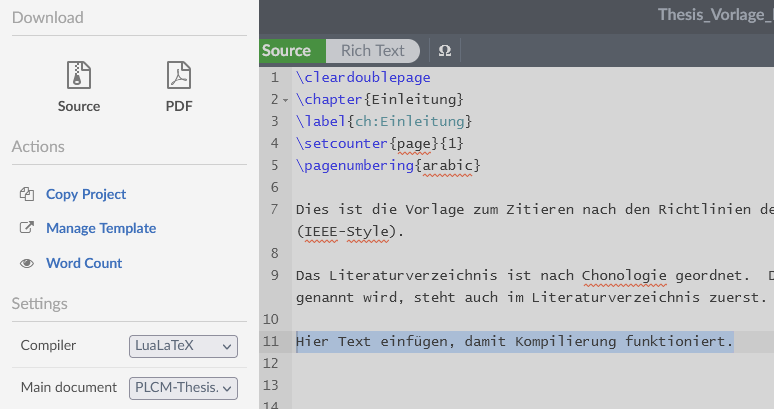
\includegraphics[width=\textwidth]{Bilder/Kapt1/Kompilierung.png}
		\caption{\centering Kompilierungseinstellungen}
		\label{fig:Kompilierung}
	\end{center}
\end{figure}

\section{Motivation}
\label{sec:Motivation}


\section{Zielsetzung}
\label{sec:Zielsetzung}

\section{Aufbau der Arbeit}
\label{sec:Aufbau}
